%%%%%%%%%%%%%%%%%%%%%%%%%%%%%%%%%%%%%%%%%
% University Assignment Title Page 
% LaTeX Template
% Version 1.0 (27/12/12)
%
% This template has been downloaded from:
% http://www.LaTeXTemplates.com
%
% Original author:
% WikiBooks (http://en.wikibooks.org/wiki/LaTeX/Title_Creation)
%
% License:
% CC BY-NC-SA 3.0 (http://creativecommons.org/licenses/by-nc-sa/3.0/)
% 
% Instructions for using this template:
% This title page is capable of being compiled as is. This is not useful for 
% including it in another document. To do this, you have two options: 
%
% 1) Copy/paste everything between \begin{document} and \end{document} 
% starting at \begin{titlepage} and paste this into another LaTeX file where you 
% want your title page.
% OR
% 2) Remove everything outside the \begin{titlepage} and \end{titlepage} and 
% move this file to the same directory as the LaTeX file you wish to add it to. 
% Then add \input{./title_page_1.tex} to your LaTeX file where you want your
% title page.
%
%%%%%%%%%%%%%%%%%%%%%%%%%%%%%%%%%%%%%%%%%
%\title{Title page with logo}
%----------------------------------------------------------------------------------------
%	PACKAGES AND OTHER DOCUMENT CONFIGURATIONS
%----------------------------------------------------------------------------------------

\documentclass[12pt]{article}
\usepackage[english]{babel}
\usepackage[utf8x]{inputenc}
\usepackage{amsmath}
\usepackage{graphicx}
\usepackage[colorinlistoftodos]{todonotes}
\usepackage[]{algorithm2e}

\begin{document}

\begin{titlepage}

\newcommand{\HRule}{\rule{\linewidth}{0.5mm}} % Defines a new command for the horizontal lines, change thickness here

\center % Center everything on the page
 
%----------------------------------------------------------------------------------------
%	HEADING SECTIONS
%----------------------------------------------------------------------------------------

\textsc{\LARGE Université de Bordeaux}\\[1.5cm] % Name of your university/college
\textsc{\Large Traitement d'image Avancée}\\[0.5cm] % Major heading such as course name
\textsc{\large Assignment 1}\\[0.5cm] % Minor heading such as course title

%----------------------------------------------------------------------------------------
%	TITLE SECTION
%----------------------------------------------------------------------------------------

\HRule \\[0.4cm]
{ \huge \bfseries Texture Synthesis}\\[0.4cm] % Title of your document
\HRule \\[1.5cm]
 
%----------------------------------------------------------------------------------------
%	AUTHOR SECTION
%----------------------------------------------------------------------------------------

\begin{minipage}{0.4\textwidth}
\begin{flushleft} \large
\emph{Author:}\\
Jimmy \textsc{Gouraud} % Your name
\end{flushleft}
\end{minipage}
~
\begin{minipage}{0.4\textwidth}
\begin{flushright} \large
\emph{Supervisor:} \\
Aurélie \textsc{Bugeau} % Supervisor's Name
\end{flushright}
\end{minipage}\\[2cm]

% If you don't want a supervisor, uncomment the two lines below and remove the section above
%\Large \emph{Author:}\\
%John \textsc{Smith}\\[3cm] % Your name

%----------------------------------------------------------------------------------------
%	DATE SECTION
%----------------------------------------------------------------------------------------

{\large \today}\\[2cm] % Date, change the \today to a set date if you want to be precise

%----------------------------------------------------------------------------------------
%	LOGO SECTION
%----------------------------------------------------------------------------------------


\includegraphics[scale=0.25]{logo.jpg}\\ % Include a department/university logo - this will require the graphicx package
 
%----------------------------------------------------------------------------------------

\vfill % Fill the rest of the page with whitespace

\end{titlepage}

\section{Introduction}
Nous allons voir et implémenter la méthode de synthèse de texture par "Non-parametric Sampling" d'Alexei A. Efros et de Thomas K. Leung.
Cette méthode permet de synthétiser une texture pixel par pixel en analysant le voisinage local du pixel, à l'aide de l'utilisation des patchs.

\section{Texture Synthesis}
\subsection{Algorithme de synthèse de texture}
L'algorithme se découpe en 3 étapes :
\begin{enumerate}
\item Initialisation de l’image de destination à partir d’un bout de la texture (appelé «seed»)
\item Recherches des pixels à traiter
\item Traitement des pixels trouvés
\end{enumerate}

\begin{algorithm}[H]
 \KwData{texture, dest\_image, patch\_size}
 \KwResult{dest\_image fill}
 fill\_seed(texture, dest\_image)\;
 \While{dest\_image not filling}{
  pixels = find\_pixels\_unfilled(dest\_image)\;
  \For{pixel in pixels}{
  	best\_patch = find\_best\_patch(pixel, dest\_image, texture, patch\_size)\;
    pixel = best\_patch.pixel\;
  }
 }
 \caption{Pseudo Code - Texture Synthesis}
\end{algorithm}

\medbreak
Lors de l'initialisation, on va créer une image de destination de la taille désirée, puis on va "coller" en son centre une "seed", c'est-à-dire un bloc de pixels de $3\times3$ issue de la texture initiale (fonction fill\_seed(texture, dest\_image)) que l'on va prendre aléatoirement. \\

Ensuite, tant que l'image de destination n'est pas remplit entièrement, on va chercher les pixels à traiter et les traiter. 

\subsection{Recherche des pixels à traiter}
Pour trouver les pixels à traiter, on va, lors de l'initialisation, créer un tableau 2D appelé "masque" de la taille de l'image de destination que l'on va initialiser à 0. On va ensuite remplir les pixels correspond à la seed à 1.
Ainsi, dans lorsque l'on cherchera les pixels à traiter, il suffira de faire une dilatation de ce masque et de faire la différence avec le masque précédent (voire figure 1).

\begin{figure}[!h]
\centering
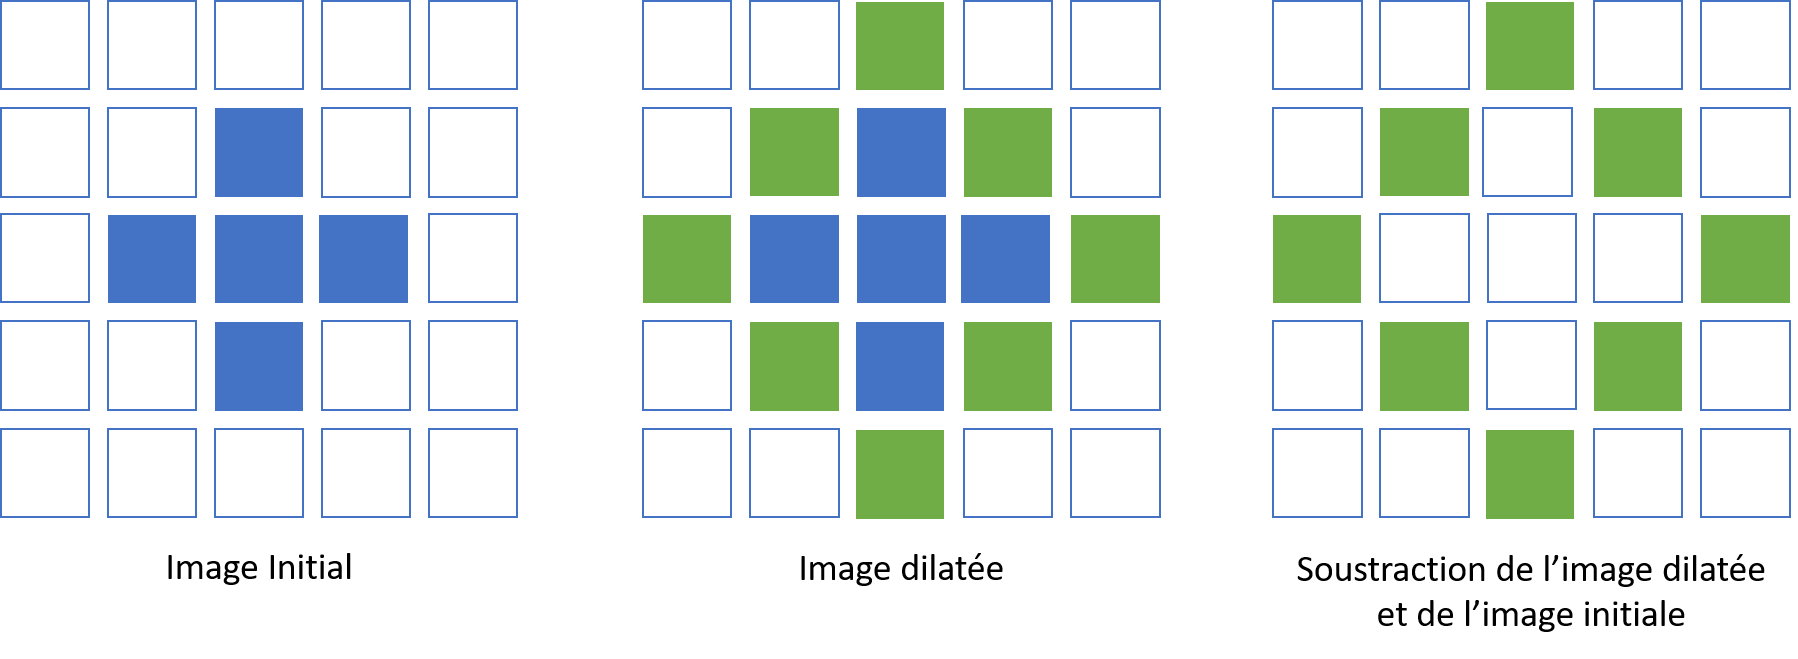
\includegraphics[scale=0.25]{dilatation_soustraction.png}
\caption{Dilatation et soustraction}
\end{figure}

On pourrait améliorer le procédé en maximisant le nombre de voisins pour chaque pixel par exemple.

\subsection{Traitement des pixels}
Pour traiter un pixel, nous allons analyser son voisinage à l'aide des patchs et essayer de trouver un environnement le plus proche possible dans notre texture initiale. Pour comparer deux patchs entre eux, nous allons avoir recours à la SSD (\textit{Sum of Squared Differences}). La SSD dans notre cas se fera sur les canaux RGB. On aurait pu de plus faire passer un noyau de convolution gaussien pour avantager les pixels proche du centre, mais les résultats ne sont pas forcément meilleurs.
\\
Après avoir parcouru l'ensemble des patchs contenue dans notre texture et les avoir comparé avec notre patch centré autour du pixel que l'on est en train de traiter, on 
sélectionne le meilleur patch. Le meilleur patch est simplement celui avec lequel on obtient la plus petite SSD. 
\\
Il suffit ensuite de recopier le pixel du centre du patch sélectionné, dans le pixel de notre image de destination.
\\
Afin d'obtenir plus de diversité dans notre génération de texture, on pourrait sélectionner aléatoirement un patch parmi les 5 meilleurs patchs par exemple, parmi tous les patchs qui possède une $SSD < min(SSD) * 1.1$.

\begin{figure}[!h]
\centering
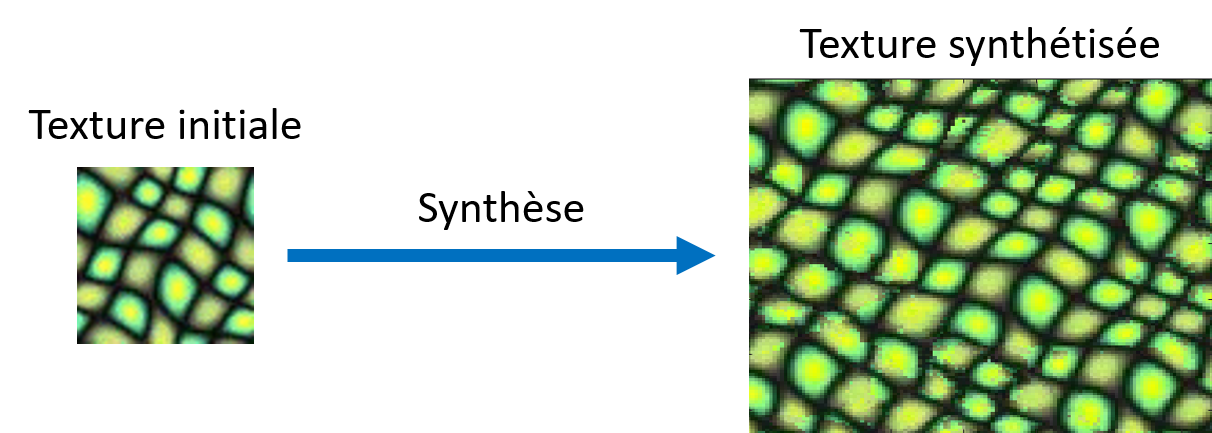
\includegraphics[scale=0.6]{synthese_de_texture.png}
\caption{Synthèse de Texture}
\end{figure}

\subsection{Modification pour faire du \textit{in painting}"}
La méthode d'\textit{in painting} permet de combler les occlusions d'une image et/ou de supprimer des éléments indésirables (comme par exemple une personne sur une photo).
\\
Le procédé pour faire du "in painting" est exactement le même que pour la synthèse de texture. On va simplement passer l'image que l'on souhaite retoucher, un masque de la taille de l'image avec comme valeur 1 les pixels que l'on souhaite garder et 0 ce que l'on souhaite traiter, et la taille d'un patch. Ensuite, au lieu de rechercher les patchs dans notre texture comme on faisait pour la méthode \textit{texture synthesis}, on va rechercher les patchs contenu directement dans notre image de destination. Ainsi on va ainsi pouvoir remplir les occlusions identifiés par le masque.

\begin{figure}[!h]
\centering
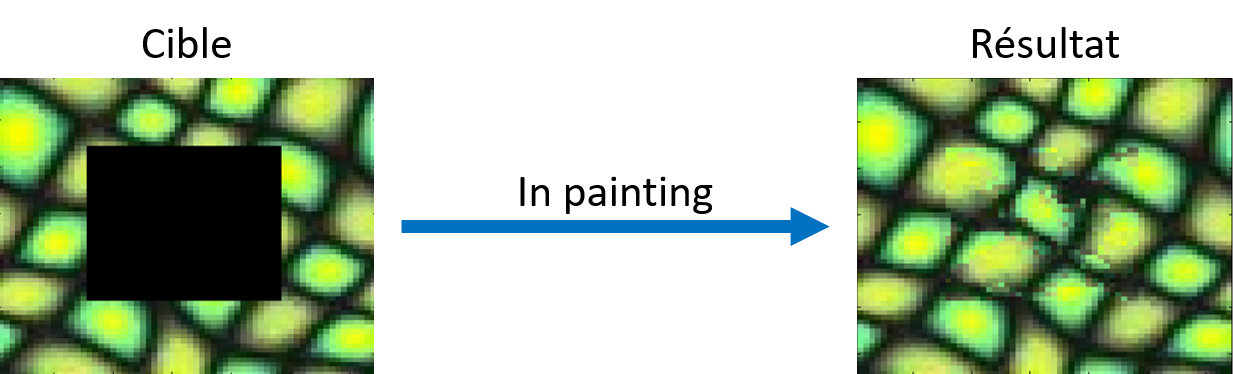
\includegraphics[scale=0.6]{inpainting.png}
\caption{In painting}
\end{figure}

\newpage
\section{Conclusion}
Pour obtenir des résultats cohérents, c'est-à-dire une texture à la fois différente mais visuellement ressemblante, il faut réussir à trouver une bonne taille de patch. Plus le patch est grand, plus la texture synthétisée ressemblera à la texture initiale, mais en contrepartie, cela entraînera du bruit dû à une plus grande diversité dans le choix du meilleur patch et donc provoquera du bruit.\cite{inpainting} \cite{tsynthesis}

\bibliographystyle{plain}
\bibliography{biblio}

\end{document}